\section{Durchführung}
\label{sec:Durchführung}

Der Versuch wird mit einer Kupfer-Röntgenröhre durchgeführt.
Diese ist auf einen schwenkbaren LiF- Kristall ausgerichtet.
Das Geiger-Müller-Zählrohr ist über einem Arm drehbar gelagert und kann unabhängig von dem Kristall gedreht werden.
Es sind somit unabhängige und gekoppelte Bewegungen möglich.
Der Aufbau ist in Abbildung \ref{fig:Aufbau} zu sehen.

\begin{figure}
  \centering
  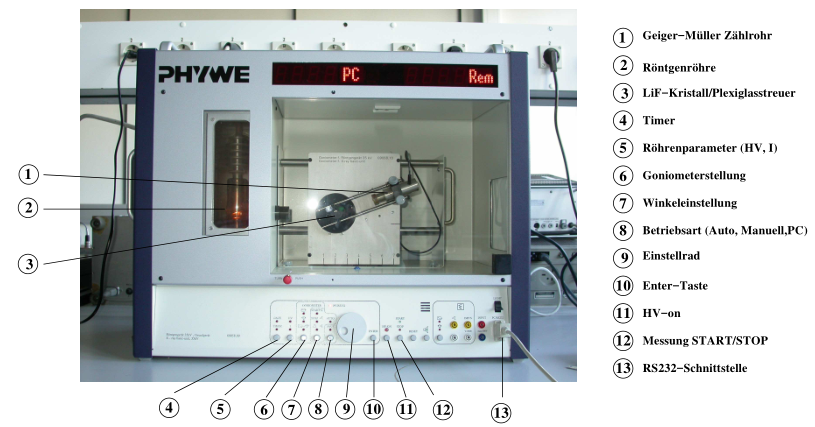
\includegraphics[width=\textwidth]{images/Aufbau.png}
  \caption{Die für die Messungen verwendete Apparatur, entnommen der Veruchsanleitung\cite[4]{sample}.}
  \label{fig:Aufbau}
\end{figure}

Die Einstellungen und Messungen werden an einem Computer durchgeführt.
Dort kann die Messart, der Drehmodus, der Kristallwinkel und die Integrationszeit eingestellt werden.
Die Messart wird auf Spektren eingestellt.
Die Beschleunigungsspannung U$_{\text{B}} = \SI{35}{\kilo\volt}$ wird für alle Messungen eingestellt.
Gleiches gilt für den Emissionsstrom von I$ = \SI{1}{\milli\ampere}$.
Die Messungen erfolgen dann automatisch.
Es sollte für jede Messungen die $\SI{1}{\milli\metre}$ Schlitzblende vor dem Geiger-Müller-Zählrohr angebracht und waagerecht ausgerichtet sein.

Um die Bragg Bedingung überprüfen zu können, wird der LiF-Kristall auf einen festen Kristallwinkel von $\SI{14}{\degree}$ eingestellt und die Intensität gemessen.
Die Integrationszeit beträgt $\Delta t = \SI{5}{\second}$.
Die Messung erfolgt im Winkelbereich von $\SI{26}{\degree}$ bis $\SI{30}{\degree}$ mit einem Winkelzuwachs von $\SI{0.1}{\degree}$

Das Emissionsspektrum der Cu-Röntgenröhre wird im 2:1 Koppelmodus durchgeführt.
Die Drehung des Kristalls ist somit mit dem der des Geiger-Müller-Zählrohrs verknüpft.
Das Röntgenspektrum der Beugungsordnung $n=1$ wird in einem Winkelbereich von $\SI{4}{\degree}$ bis $\SI{26}{\degree}$ in $\SI{0.2}{\degree}$ Schritten gemessen.
Hierbei beträgt die Integrationszeit $\SI{5}{\second}$.

Um die Absorptionsspektren von verschiedenen Materialen zu messen, werden Blenden aus dem zu untersuchenden Material vor das Geiger-Müller-Zählrohr geschraubt.
Die zu untersuchenden sind Brom, Strontium, Zink und Zirkonium.
Der Winkelbereich wird dabei so gewählt, dass die spezifischen K-Kanten im Winkelbereich liegen.
Die Winkelbereiche lauten nun:

\begin{align*}
  \text{Brom} &: \SI{24}{\degree} \leq \theta \leq \SI{28}{\degree} \\
  \text{Strontium} &: \SI{21}{\degree} \leq \theta \leq \SI{25}{\degree} \\
  \text{Zink} &: \SI{35}{\degree} \leq \theta \leq \SI{39}{\degree} \\
  \text{Zirkonium} &: \SI{19}{\degree} \leq \theta \leq \SI{23}{\degree}
\end{align*}

Diese Bereiche werden in $\SI{0.1}{\degree}$ Schritten abgefahren.
Die Messzeit beträgt $\SI{10}{\second}$.
Dies wird für Bismut wiederholt, nur ist hier der Winkelbereich größer gewählt worden, da hier die L-Kanten untersucht werden sollen.
Alle anderen Einstellungen bleiben gleich
Der Bereich lautet:

\begin{align*}
  \text{Zink} &: \SI{22}{\degree} \leq \theta \leq \SI{30}{\degree}
\end{align*}
\FloatBarrier
